\documentclass[12pt]{article}
\usepackage{graphicx}
\usepackage[left=3cm,top=3cm,right=3cm,bottom=3cm]{geometry}

\begin{document}

\title{Extended Bayesian Skyline Plot Tutorial}

\author{Alexei J Drummond, Joseph Heled and Walter Xie}

\date{\today{}}

\maketitle

\section*{Introduction}

This practical will take you though the estimation of population history of a virus epidemic using the extended Bayesian skyline plot.

To undertake the exercises in this practical, you will need to have access to the following software packages in a format that is compatible with your
computer system (all three are available for Mac OS X, Windows and Linux/UNIX operating systems):

\begin{itemize}

\item {\bf BEAST} - this package contains the BEAST program, BEAUti, TreeAnnotator and other utility programs. At the time of writing, the
current version is v1.6.2. It is available for download from \texttt{http://beast.bio.ed.ac.uk/} and \texttt{http://code.google.com/p/beast-mcmc/downloads/list}.
\item {\bf Tracer} - this program is used to explore the output of BEAST (and other Bayesian MCMC programs). It graphically and
quantitively summarizes the distributions of continuous parameters and provides diagnostic information. At the time of
writing, the current version is v1.5. It is available for download from \texttt{http://tree.bio.ed.ac.uk/software/tracer/}.
\item {\bf FigTree} - this is an application for displaying and printing molecular phylogenies, in particular those obtained using
BEAST. At the time of writing, the current version is v1.3.1. It is available for download from \texttt{http://tree.bio.ed.ac.uk/\\software/figtree/}.
\end{itemize}


%%%%%%%%%%%%%%%%%%%%%%%%%%%%%%%%%%%%%%%%%%%%%
%%%
%%% EXERCISE 3 - BAYESIAN SKYLINE PLOT
%%%
%%%%%%%%%%%%%%%%%%%%%%%%%%%%%%%%%%%%%%%%%%%%%

In this exercise we will investigate the population history of the the H5N1 influenza epidemic, by using the Extended Bayesian Skyline Plot (EBSP), which estimates changes in effective population size through time. The data are 21 H5N1 strain Influenza A sequences sampled between 1997 and 2005 from Southeast Asia; including viruses from birds, pigs and humans.

\section*{BEAUti }

The program BEAUti is a user-friendly program for setting the
model parameters for BEAST. Run BEAUti by double clicking on its icon. 

\subsection*{Loading the NEXUS file }

To load a NEXUS format alignment, simply select the \texttt{Import
Alignment...} option from the File menu: 

\medskip{}

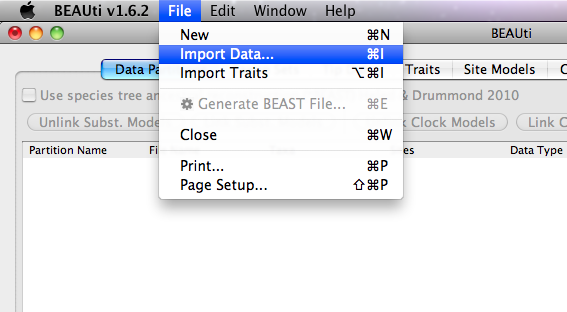
\includegraphics[scale=0.5]{figures/ImportNexus}

\medskip{}

Select the file called \texttt{Flu.nex}. This file contains an alignment of 21 sequences from the Influenza A virus, 1698 nucleotides in length. 

\medskip{}

Once loaded, the list of taxa and the actual alignment will be displayed
in the main panel:

\medskip{}

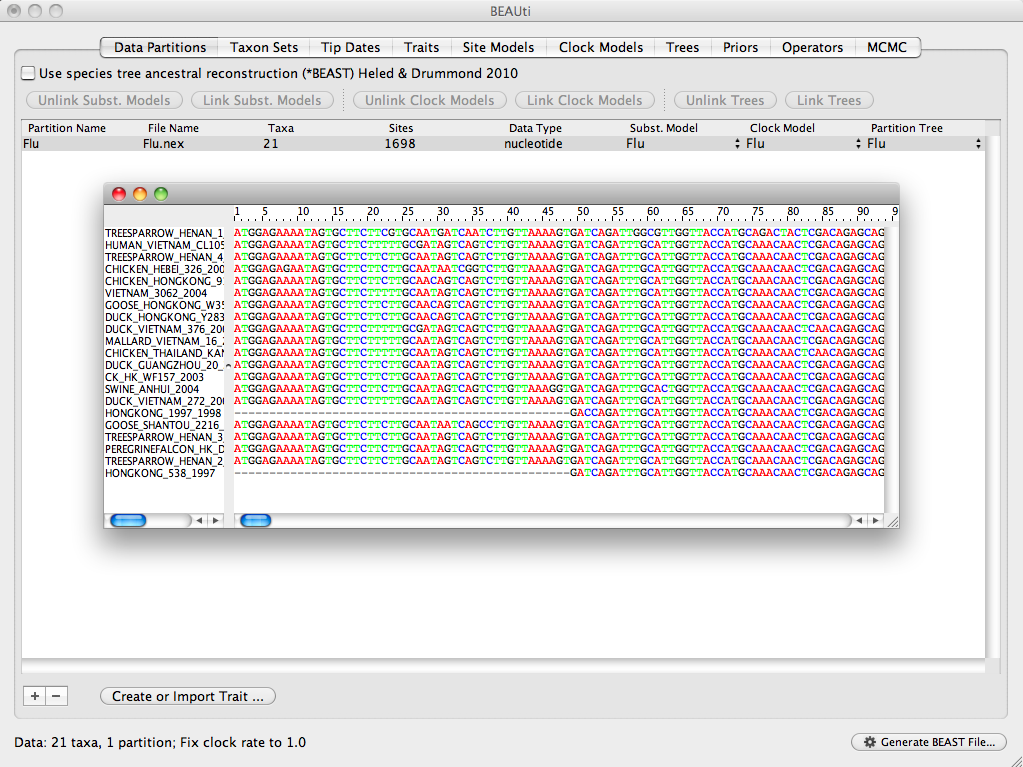
\includegraphics[scale=0.4]{figures/BEAUti_Data}

\medskip{}


\subsection*{Tip Dates}

Click on the {\bf Tip Dates} tab at the top of the
main window, and check the checkbox {\bf Use tip dates}. By default all the taxa are assumed to have a date of zero (i.e. the sequences are assumed to be sampled at the same time).
In this case, the Influenza sequences have been sampled at various dates going back to 1997. The actual year of sampling
is given in the name of each taxon and we could simply edit the value in the Date column of the table to reflect these.
However we can also use the Guess Dates facility by clicking {\bf Guess Dates} button. In the {\bf Guess Dates for Taxa} dialog box, select \texttt{last} in the drop down and type underscore in {\bf Prefix}, then click the {\bf OK} button. The dates will appear in the appropriate column of the main window. You can then check these and edit them manually if required. 

\medskip{}

\frame{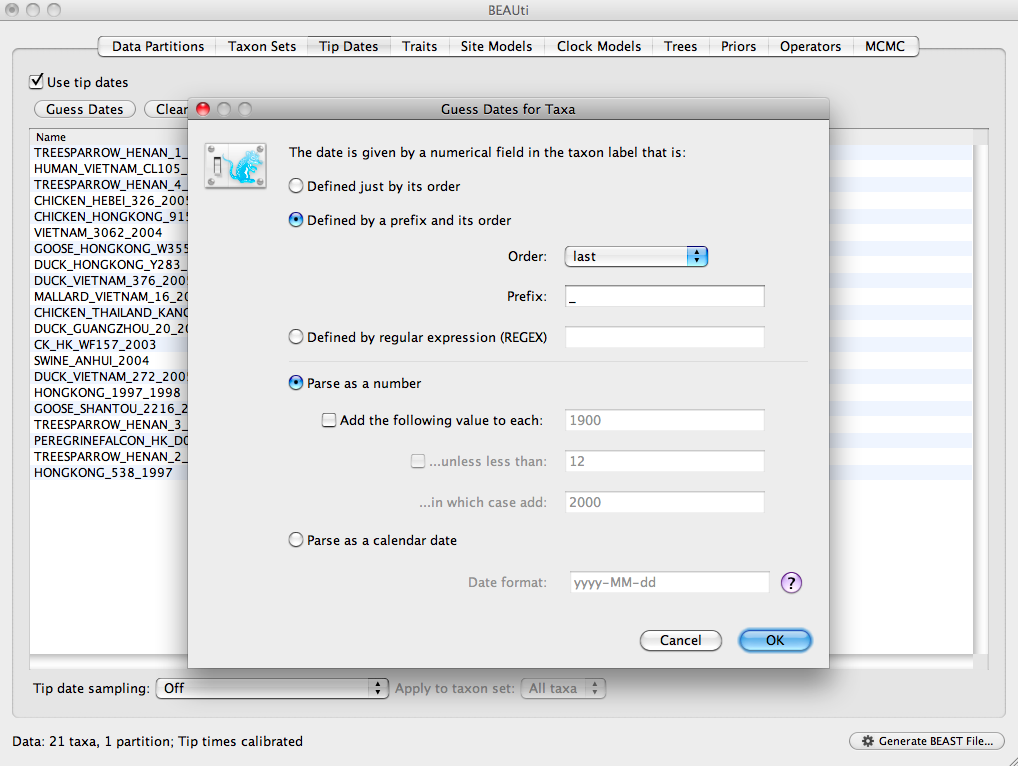
\includegraphics[scale=0.4]{figures/BEAUTi_TipDates}}

\medskip{}


\subsection*{Setting the substitution model}

The next thing to do is to click on the {\bf Site Models} tab at the top of the
main window. This will reveal the evolutionary model settings for
BEAST. Exactly which options appear depend on whether the data are
nucleotides or amino acids.
The settings that will appear after loading data set will
be the default values so we need to make some changes. 

Most of the models should be familiar to you. For this analysis, we
will make three changes. First, select \textbf{Empirical} under the \textbf{Base
frequencies} menu. Second, select the {\bf 3 partitions: codon positions 1, 2, 3} option so that each codon position has its own rate of evolution. For more information about linking/unlinking model parameters across codon positions see the Notes.
\medskip{}

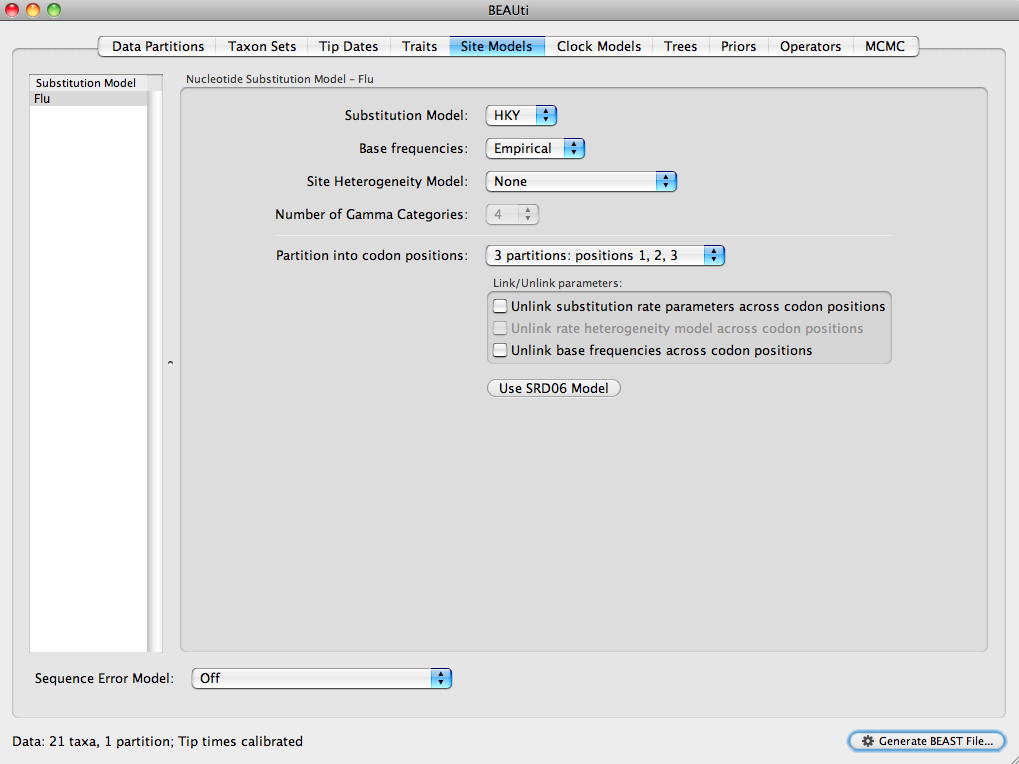
\includegraphics[scale=0.4]{figures/BEAUti_Subst_Model}

\medskip{}

\subsection*{Setting the clock model}

The third thing we will do is to click on the {\bf Clock Models} tab at the top of the
main window, and to change the molecular clock model to \textbf{Relaxed Clock: Uncorrelated
Log-normal} so as to account for lineage-specific rate heterogeneity.
Your model options should now look like this: 

\medskip{}

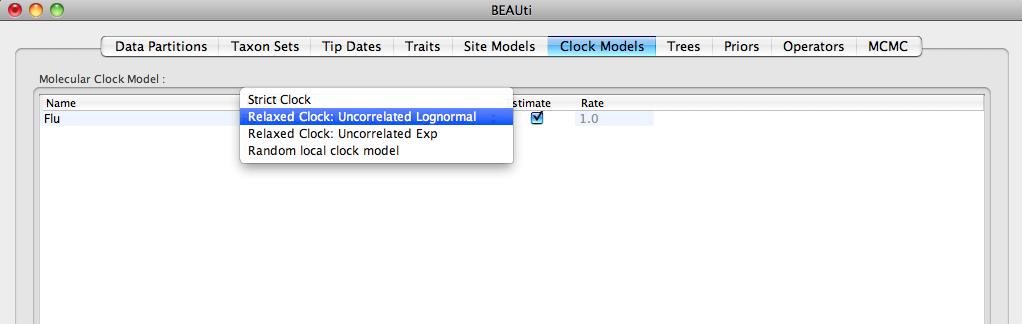
\includegraphics[scale=0.4]{figures/BEAUti_Clock_Model}

\medskip{}

The \textbf{Estimate} check box is required to be checked. This is because we wish to estimate
the clock rate (and in doing so the divergence times). But this will be automatically checked, in this case, when we checked the checkbox {\bf Use tip dates} in \textbf{Tip Dates} panel.


\section*{Trees}

The {\bf Trees} tab allows priors to be specified for each parameter in the
model. The first thing to do is to select {\bf Coalescent: Extended Bayesian Skyline Plot} from the {\bf Tree prior} dropdown menu, and leave the {\bf Model Type} as default.

\medskip{}

\frame{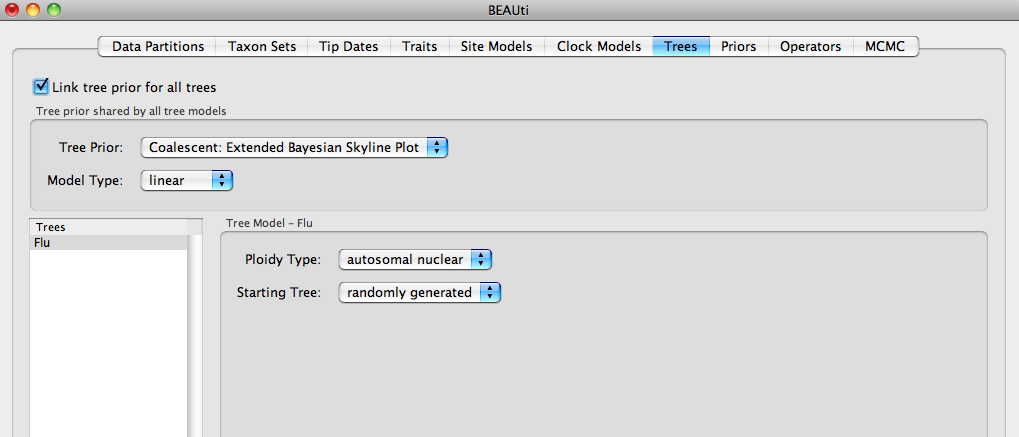
\includegraphics[scale=0.4]{figures/BEAUTi_Tree}}

\medskip{}


\subsection*{Priors }

Define the prior not specified (marked as red colour), and the priors table should now look like this: 

\medskip{}

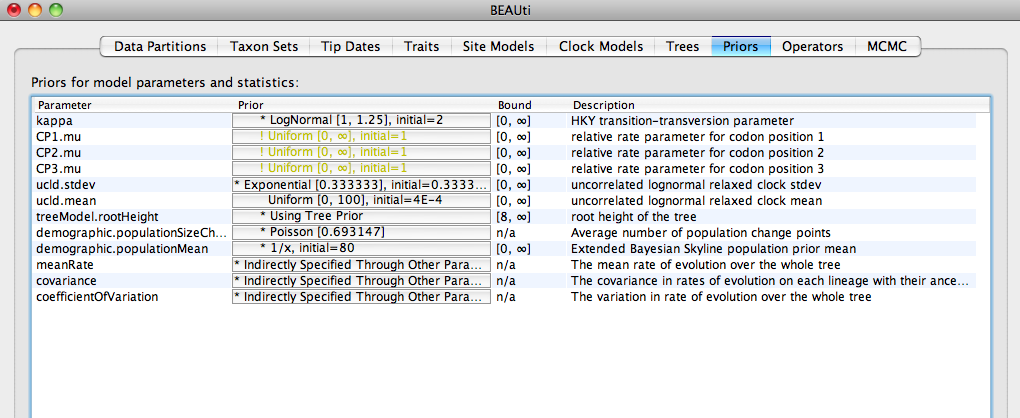
\includegraphics[scale=0.4]{figures/BEAUti_Prior}

\medskip{}


\section*{Setting the MCMC options}

For this dataset let's initially set the chain length to 3,000,000. This will take 5-10 minutes on a fast computer. Set the two sampling frequencies to 3000 and 1000 respectively.

\medskip{}

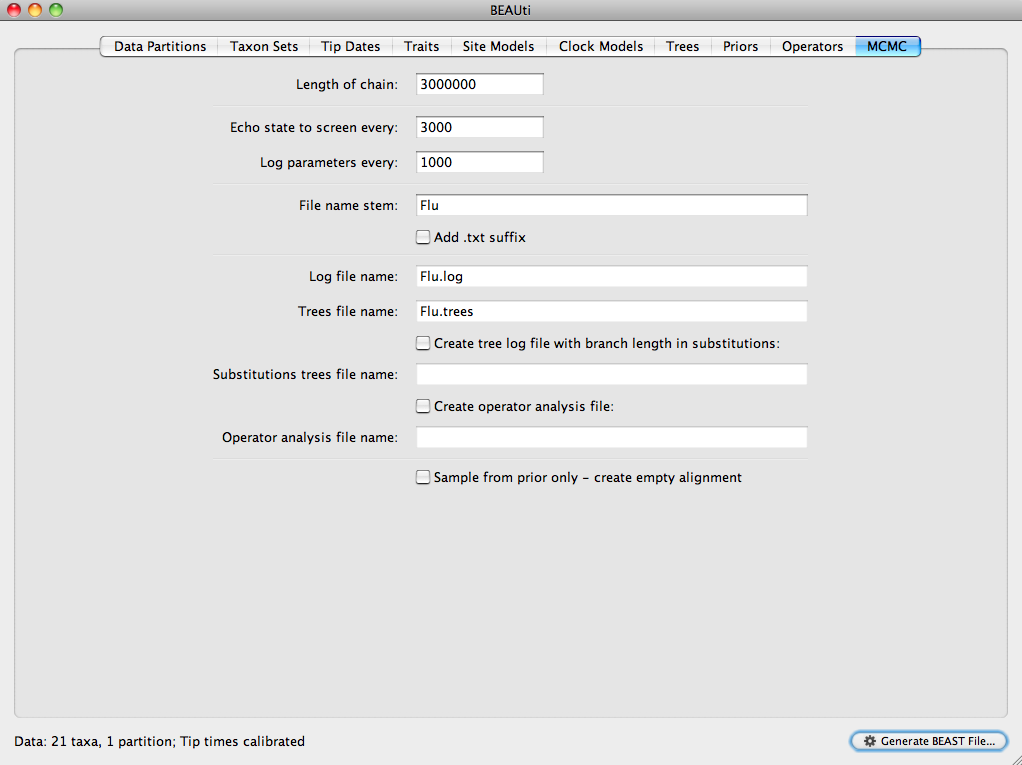
\includegraphics[scale=0.4]{figures/BEAUti_MCMC}

\medskip{}

We are now ready to create the BEAST XML file. To do this,
either select the {\bf Generate BEAST File...} option from the File menu or click the similarly labelled button at the bottom of the
window. Save the file with an appropriate name
(we usually end the filename with \texttt{.xml}, i.e., \texttt{Flu.xml}).
We are now ready to run the file through BEAST.  


\section*{Running BEAST}

Now run BEAST and when it asks for an input file, provide your newly
created XML file as input. 

\medskip{}

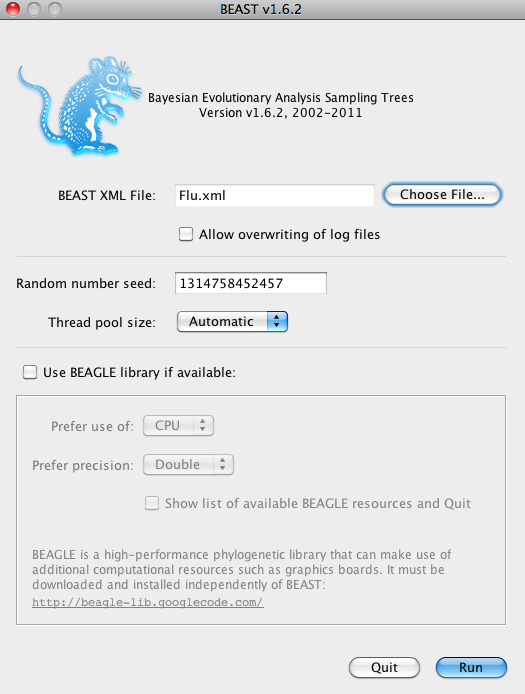
\includegraphics[scale=0.4]{figures/BEAST}

\medskip{}

BEAST will then run until it has finished
reporting information to the screen. The actual results files are
save to the disk in the same location as your input file. The output to the screen will
look something like this: 

{\scriptsize   
\begin{verbatim}

                  BEAST v1.6.2, 2002-2011
       Bayesian Evolutionary Analysis Sampling Trees
                 Designed and developed by
   Alexei J. Drummond, Andrew Rambaut and Marc A. Suchard
                              
               Department of Computer Science
                   University of Auckland
                  alexei@cs.auckland.ac.nz
                              
             Institute of Evolutionary Biology
                  University of Edinburgh
                     a.rambaut@ed.ac.uk
                              
              David Geffen School of Medicine
           University of California, Los Angeles
                     msuchard@ucla.edu
                              
                Downloads, Help & Resources:
                 	http://beast.bio.ed.ac.uk
                              
Source code distributed under the GNU Lesser General Public License:
            	http://code.google.com/p/beast-mcmc
                              
                     BEAST developers:
	Alex Alekseyenko, Erik Bloomquist, Joseph Heled, Sebastian Hoehna, 
	Philippe Lemey, Wai Lok Sibon Li, Gerton Lunter, Sidney Markowitz, 
	Vladimir Minin, Michael Defoin Platel, Oliver Pybus, Chieh-Hsi Wu, 
                        	Walter Xie
                              
                         Thanks to:
    	Roald Forsberg, Beth Shapiro and Korbinian Strimmer


Random number seed: 1314758452457

Parsing XML file: Flu.xml
  File encoding: MacRoman
Read alignment: alignment
  Sequences = 21
      Sites = 1698
   Datatype = nucleotide
INFO: resetting length of parameter demographic.popSize(size 1) in variable demographic model to 21
INFO: resetting length of parameter demographic.indicators in variable demographic model to 20
Creating the tree model, 'treeModel'
  initial tree topology = ((((((((CHICKEN_HEBEI_326_2005,MALLARD_VIETNAM_16_2003),(CK_HK_WF157_2003,GOOSE_HONGKONG_W355_1997)),DUCK_HONGKONG_Y283_1997),(DUCK_GUANGZHOU_20_2005,VIETNAM_3062_2004)),PEREGRINEFALCON_HK_D0028_2004),(DUCK_VIETNAM_272_2005,HONGKONG_538_1997)),(CHICKEN_HONGKONG_915_1997,TREESPARROW_HENAN_1_2004)),((((((GOOSE_SHANTOU_2216_2005,TREESPARROW_HENAN_2_2004),DUCK_VIETNAM_376_2005),TREESPARROW_HENAN_3_2004),(HUMAN_VIETNAM_CL105_2005,TREESPARROW_HENAN_4_2004)),SWINE_ANHUI_2004),(CHICKEN_THAILAND_KANCHANABURI_CK_160_2005,HONGKONG_1997_1998)))
  tree height = 247.15904555133568
Variable demographic: linear control points
Using discretized relaxed clock model.
  over sampling = 1
  parametric model = logNormalDistributionModel
   rate categories = 40
Creating state frequencies model: Using empirical frequencies from data = {0.34816, 0.18626, 0.22924, 0.23635}
Creating HKY substitution model. Initial kappa = 2.0
Creating site model.
  with initial relative rate = 1.0
Creating site model.
  with initial relative rate = 1.0
Creating site model.
  with initial relative rate = 1.0
Loading native NucleotideLikelihoodCore successfully from /Users/walter/Documents/BEAST1release/BEAST 1.6.2
TreeLikelihood(treeModel) using native nucleotide likelihood core
  Ignoring ambiguities in tree likelihood.
  With 70 unique site patterns.
Branch rate model used: discretizedBranchRates
TreeLikelihood(treeModel) using native nucleotide likelihood core
  Ignoring ambiguities in tree likelihood.
  With 59 unique site patterns.
Branch rate model used: discretizedBranchRates
TreeLikelihood(treeModel) using native nucleotide likelihood core
  Ignoring ambiguities in tree likelihood.
  With 148 unique site patterns.
Branch rate model used: discretizedBranchRates
Parameter weights for delta exchange are: 566	566	566	
Creating swap operator for parameter branchRates.categories (weight=10.0)
Likelihood is using -1 threads.
Creating the MCMC chain:
  chainLength=3000000
  autoOptimize=true
  autoOptimize delayed for 30000 steps
# BEAST v1.6.2, Build r4230
# Generated Wed Aug 31 14:41:17 NZST 2011 [seed=1314758452457]
state	Posterior   	Prior       	Likelihood  	rootHeight  	ucld.mean   
0	-8308.4293  	-231.1869   	-8077.2425  	247.159     	4E-4        	-
3000	-4701.8333  	-240.6039   	-4461.2294  	93.2771     	2.79052E-4  	-
6000	-4651.8852  	-251.9135   	-4399.9717  	116.700     	1.95435E-4  	-
9000	-4626.2601  	-233.4174   	-4392.8427  	57.6287     	3.98442E-4  	-
12000	-4627.0052  	-240.3684   	-4386.6368  	65.3081     	3.92572E-4  	0.04 hours/million states

... ...

2988000	-4487.6260  	-123.3019   	-4364.3241  	8.45464     	4.92124E-3  	0.03 hours/million states
2991000	-4491.1004  	-122.0603   	-4369.0401  	8.91219     	4.88611E-3  	0.03 hours/million states
2994000	-4497.3501  	-124.6421   	-4372.7080  	9.51158     	3.84217E-3  	0.03 hours/million states
2997000	-4476.0401  	-113.6861   	-4362.3541  	8.30970     	4.01222E-3  	0.03 hours/million states
3000000	-4470.6685  	-108.1633   	-4362.5052  	8.47905     	4.56921E-3  	0.03 hours/million states

Operator analysis
Operator                                          Tuning   Count      Time     Time/Op  Pr(accept) 
scale(kappa)                                      0.483   1785       396      0.22     0.2941      
allMus                                            0.446   54044      8514     0.16     0.2099      
scale(ucld.mean)                                  0.701   53768      12100    0.23     0.2515      
scale(ucld.stdev)                                 0.302   53775      12081    0.22     0.3731      
subtreeSlide(treeModel)                           2.844   269507     26761    0.1      0.0821      
Narrow Exchange(treeModel)                                269915     22087    0.08     0.0822      
Wide Exchange(treeModel)                                  54109      2343     0.04     0.0069      
wilsonBalding(treeModel)                                  54007      5907     0.11     0.0045      
scale(treeModel.rootHeight)                       0.686   54204      3861     0.07     0.1719      
uniform(nodeHeights(treeModel))                           539257     63937    0.12     0.3729      
scale(demographic.populationMean)                 0.374   54301      2783     0.05     0.2988      
SampleNonActive(demographic.indicators)                   270452     15308    0.06     1.0         
bitFlip(demographic.indicators)                           538852     31201    0.06     0.0299      
scale(demographic.popSize)                        0.234   108409     6145     0.06     0.254       
up:ucld.mean down:nodeHeights(treeModel)          0.957   53647      6615     0.12     0.0844      
swapOperator(branchRates.categories)                      180128     23326    0.13     0.7171      
randomWalkInteger(branchRates.categories)                 179485     19232    0.11     0.9756      
uniformInteger(branchRates.categories)                    180355     19256    0.11     0.7996      

5.749666666666667 minutes 

\end{verbatim}}



\section*{Analysing the BEAST output}

You can overlay the density plots of multiple logged quantities in order to compare them (it is up to the user to determine whether they are comparable on the the same axis or not). Select the relative substitution rates for all three codon positions in the table to the left (labelled
\texttt{CP1.mu}, \texttt{CP2.mu} and \texttt{CP3.mu}). You will now see the posterior probability densities for the relative
substitution rate at all three codon positions overlaid:

\medskip{}

\frame{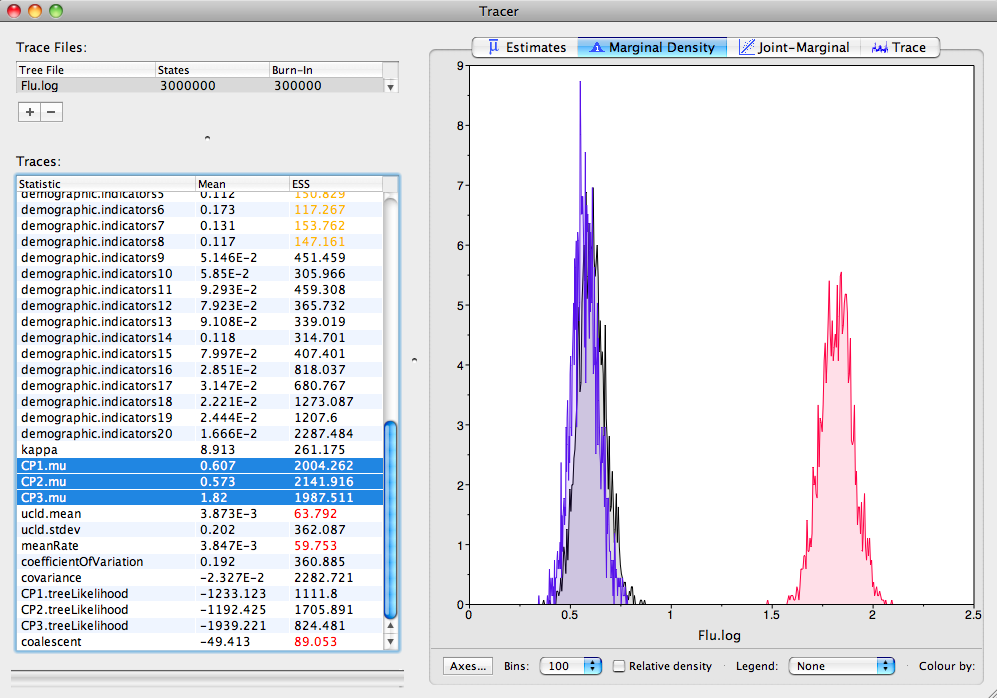
\includegraphics[scale=0.40]{figures/Tracer_relativeRates}}

\medskip{}

This plot clearly shows that the evolution of these sequences is dominated by purifying selection as the 3rd codon position (known as the wobble position) has a much higher rate of evolution (about 3 times faster) than either of the other codon positions.

\section*{Constructing the extended Bayesian skyline plot}

To construct the EBSP simply select {\bf Extended Bayesian Skyline Reconstruction...} from the {\bf Analysis} menu. Select the appropriate trees log file (e.g. \texttt{Flu.trees}) that corresponds to the parameter log file loaded in Tracer. The remaining default values in the dialog box will be fine, so click OK. 

\medskip{}

\frame{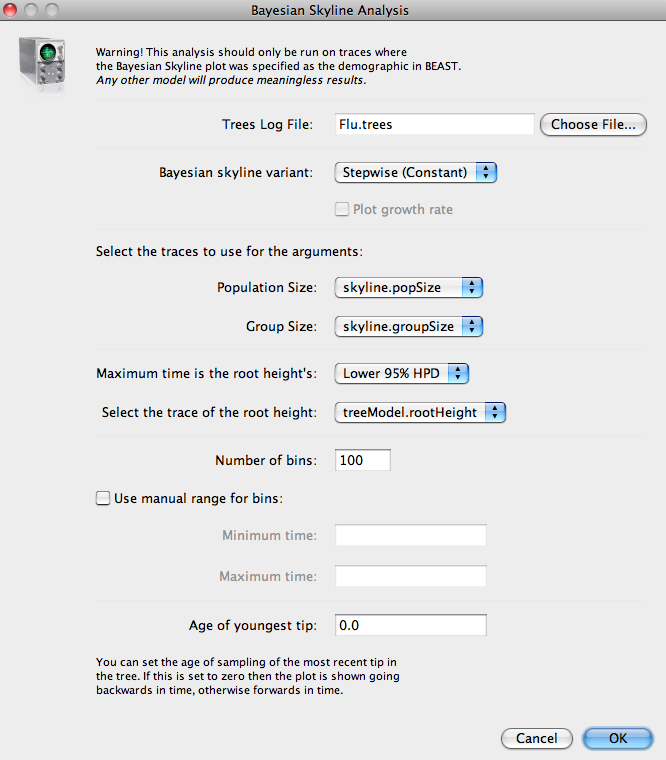
\includegraphics[scale=0.4]{figures/Tracer_BSP_dialog}}

\medskip{}

After the trees file is processed the EBSP should appear in a new window:

\medskip{}

\frame{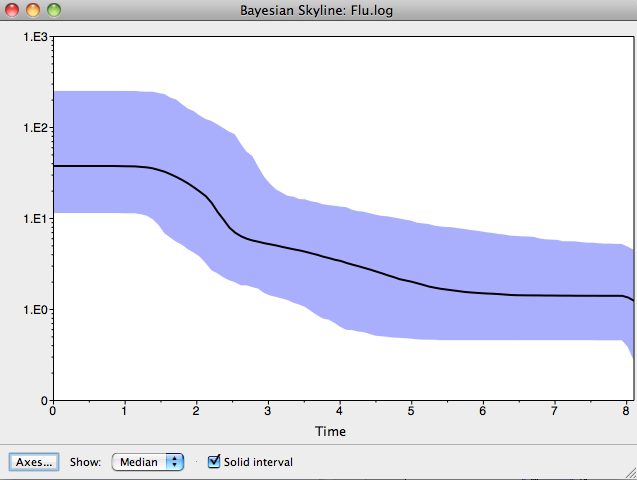
\includegraphics[scale=0.5]{figures/Tracer_BSP}}

\medskip{}

\newpage

\subsection*{Questions}

\textit{By what amount did the effective population size of H5N1 Influenza grow from 1997 to 2005 according to the EBSP?}
 
 \vspace{5 mm}
 \framebox(420,30){}
   \vspace{5 mm}

\textit{What are the underlying assumptions of the EBSP? Are the violated by this data set?}
 
 \vspace{5 mm}
 \framebox(420,90){}
   \vspace{5 mm}

\newpage

\section*{Summarizing the trees}

BEAST also produces a sample of plausible trees along its sample of parameter estimates. 
These need to be summarized
using the program {\bf TreeAnnotator} (see Notes for details). This will take the set of trees and find the best
supported one. It will then annotate this summary tree with the mean ages of all the
nodes and the HPD ranges. It will also calculate the posterior clade probability for each
node. Run the TreeAnnotator program and set it up to look like this:

\medskip{}

\frame{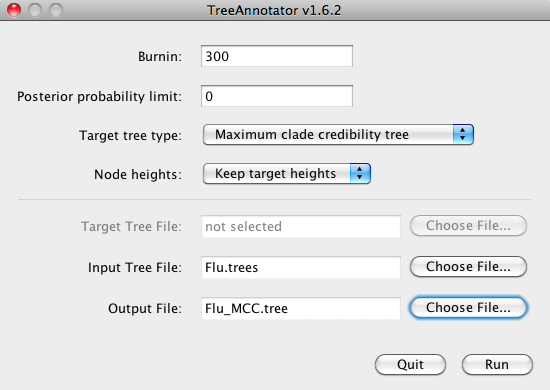
\includegraphics[scale=0.5]{figures/TreeAnnotator}}

\medskip{}


And view it in {\bf FigTree}:

\medskip{}

\frame{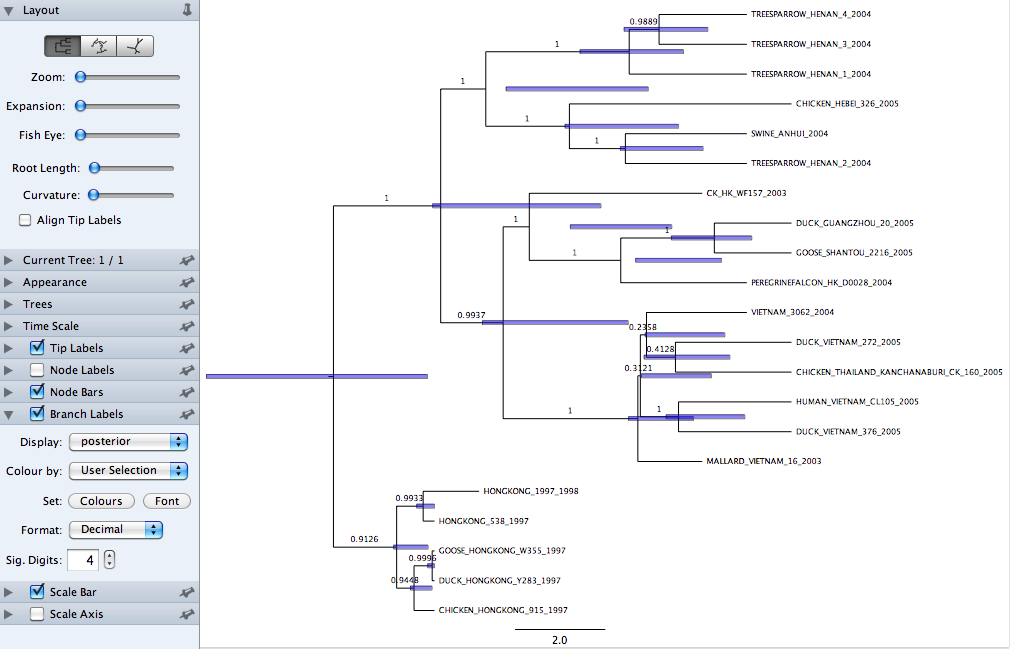
\includegraphics[scale=0.4]{figures/Figtree}}

\medskip{}

\section*{Conclusion and Resources}
This practical only scratches the surface of the analyses that are possible to undertake using BEAST. It has hopefully provided
a relatively gentle introduction to the fundamental steps that will be common to all BEAST analyses and provide a basis for
more challenging investigations. BEAST is an ongoing development project with new models and techniques being added
on a regular basis. The BEAST website provides details of the mailing list that is used to announce new features and to
discuss the use of the package. The website also contains a list of tutorials and recipes to answer particular evolutionary
questions using BEAST as well as a description of the XML input format, common questions and error messages.

\begin{itemize}
\item The BEAST website: \texttt{http://beast.bio.ed.ac.uk/}
\item Tutorials: \texttt{http://beast.bio.ed.ac.uk/Tutorials/}
\item Frequently asked questions: \texttt{http://beast.bio.ed.ac.uk/FAQ/}
\end{itemize}

\section*{Notes}

This section has some extra details about aspects of some of the programs.

\subsection*{Guess Dates}

This operation attempts to guess what the dates are from information contained within the taxon names. It works by trying to
find a numerical field within each name. If the taxon names contain more than one numerical field (such as the RSVA
sequences in Exercise 2) then you can specify how to find the one that corresponds to the date of sampling. You can either
specify the order that the date field comes (e.g., first, last or various positions in between) or specify a prefix (some
characters that come immediately before the date field in each name). For the RSVA sequences you can select `last' from
the drop-down menu for the order or use the prefix option and specify `\_' (underscore) as the prefix.

In this dialog box, you can also get BEAUti to add a fixed value to each guessed date. In this case the value ``1900'' has
been added to turn the dates from 2 digit years to 4 digit. Any dates in the taxon names given as ``00'' would thus become
``1900''. Some of the sequences in the example file actually have dates after the year 2000 so selecting the will option would
convert them correctly, adding 2000 to any date less than 09. When you press OK the dates will appear in the appropriate
column of the main window. You can then check these and edit them manually as required. At the top of the window you
can set the units that the dates are given in (years, months, days) and whether they are specified relative to a point in the
past (as would be the case for years such as 1984) or backwards in time from the present (as in the case of radiocarbon
ages).

\subsection*{Operators}
Each parameter in the model has one or more ``operators'' (these are variously called moves and proposals by other MCMC
software packages such as MrBayes and LAMARC). The operators specify how the parameters change as the MCMC runs.
The operators tab in BEAUti has a table that lists the parameters, their operators and the tuning settings for these operators.
In the first column are the parameter names. These will be called things like \texttt{kappa} which means the HKY model's
kappa parameter (the transition-transversion bias). The next column has the type of operators that are acting on each
parameter. For example, the scale operator scales the parameter up or down by a proportion, the random walk operator
adds or subtracts an amount to the parameter and the uniform operator simply picks a new value uniformly within a range.
Some parameters relate to the tree or to the divergence times of the nodes of the tree and these have special operators.

The next column, labelled {\bf Tuning}, gives a tuning setting to the operator. Some operators don't have any tuning settings so
have {\bf n/a} under this column. The tuning parameter will determine how large a move each operator will make which will affect
how often that change is accepted by the MCMC which will affect the efficency of the analysis. For most operators (like
random walk and subtree slide operators) a larger tuning parameter means larger moves. However for the scale operator a
tuning parameter value closer to 0.0 means bigger moves. At the top of the window is an option called {\bf Auto Optimize}
which, when selected, will automatically adjust the tuning setting as the MCMC runs to try to achieve maximum efficiency. At
the end of the run a table of the operators, their performance and the final values of these tuning settings will be written to
standard output. These can then be used to set the starting tuning settings in order to minimize the amount of time taken to
reach optimum performance in subsequent runs.

The next column, labelled {\bf Weight}, specifies how often each operator is applied relative to the others. Some parameters
tend to be sampled very efficiently - an example is the kappa parameter - these parameters can have their operators downweighted
so that they are not changed as often (this may mean weighting other operators up since the weights must be
integers).

\subsection*{Codon position models}

\begin{itemize}
\item Selecting the {\bf Partition into codon positions} option assumes that the data are aligned as codons. This option will then
estimate a separate rate of substitution for each codon position, or for 1+2 versus 3, depending on the setting.
Estimating rates and dates from time-sample sequences � a hands-on practical
3
\item Selecting the {\bf Unlink substitution model across codon positions} will specify that BEAST should estimate a separate
transition-transversion ratio or general time reversible rate matrix for each codon position.
\item Selecting the {\bf Unlink rate heterogeneity model across codon positions} will specify that BEAST should estimate set
of rate heterogeneity parameters (gamma shape parameter and/or proportion of invariant sites) for each codon position.
\item If there are no dates for the sequences (they are contemporaneous) then you can specify a fixed mean substitution rate
obtained from another source. Setting this to 1.0 will result in the ages of the nodes of the tree being estimated in units of
substitutions per site (i.e. the normal units of branch lengths in popular packages such as MrBayes).
\end{itemize}

\subsection*{Tracer statistics}

The statistics reported in Tracer for each logged quantity are:

\begin{itemize}
\item Mean - The mean value of the samples (excluding the burn-in).
\item Stdev - The standard error of the mean. This takes into account the effective sample size so a small ESS will give a large
standard error.
\item Median - The median value of the samples (excluding the burn-in).
95\% HPD Lower - The lower bound of the highest posterior density (HPD) interval. The HPD is the shortest interval that
contains 95\% of the sampled values.
\item 95\% HPD Upper - The upper bound of the highest posterior density (HPD) interval.
\item Auto-Correlation Time (ACT) - The average number of states in the MCMC chain that two samples have to be separated
by for them to be uncorrelated (i.e. independent samples from the posterior). The ACT is estimated from the samples in the
trace (excluding the burn-in).
\item Effective Sample Size (ESS) - The effective sample size (ESS) is the number of independent samples that the trace is
equivalent to. This is calculated as the chain length (excluding the burn-in) divided by the ACT.
\end{itemize}

\subsection*{TreeAnnotator}

The sampled trees in BEAST are written to a separate file called the `trees' file. This file is a
standard NEXUS format file. As such it can easily be loaded into other software in order to examine the trees it contains. One
possibility is to load the trees into a program such as PAUP* and construct a consensus tree in a similar manner to
summarizing a set of bootstrap trees. In this case, the support values reported for the resolved nodes in the consensus tree
will be the posterior probability of those clades.

TreeAnnotator is a software program distributed with BEAST that can summarize the tree file. 
It takes a single `target' tree and annotates it with the summarized information from the entire sample of trees.
The summarized information includes the average node ages (along with the HPD intervals), the posterior support and the
average rate of evolution on each branch (for models where this can vary). The program calculates these values for each
node or clade observed in the specified `target' tree. The options in TreeAnnotator are detailed below:

\begin{itemize}
\item {\bf Burnin} - This is the number of trees in the input file that should be excluded from the summarization. This value is given
as the number of trees rather than the number of steps in the MCMC chain. Thus for the example above, with a chain of
1,000,000 steps, sampling every 1000 steps, there are 1000 trees in the file. To obtain a 10\% burnin, set this value to
100.
\item {\bf Posterior probability limit} - This is the minimum posterior probability for a node in order for TreeAnnotator to store the
annoted information. The default is 0.5 so only nodes with this posterior probability or greater will have information
summarized (the equivalent to the nodes in a majority-rule consensus tree). Set this value to 0.0 to summarize all nodes in
the target tree.
\item {\bf Target tree type} - This has two options ``Maximum clade credibility'' or ``User target tree''. For the latter option, a
NEXUS tree file can be specified as the Target Tree File, below. For the former option, TreeAnnotator will examine every
tree in the Input Tree File and select the tree that has the highest sum of the posterior probabilities of all its nodes.
\item {\bf Node heights} - This option specifies what node heights (times) should be used for the output tree. If the ``Keep target
heights'' is selected, then the node heights will be the same as the target tree. The other two options give node heights
as an average (Mean or Median) over the sample of trees.
\item {\bf Target Tree File} - If the ``User target tree'' option is selected then you can use ``Choose File...'' to select a NEXUS file
containing the target tree.
\item I{\bf nput Tree File} - Use the ``Choose File...'' button to select an input trees file. This will be the trees file produced by
BEAST.
\item {\bf Output File} - Select a name for the output tree file.
\end{itemize}

Once you have selected all the options, above, press the ``Run'' button. 

\end{document}
